%% Creator: Inkscape 1.2.1 (9c6d41e410, 2022-07-14), www.inkscape.org
%% PDF/EPS/PS + LaTeX output extension by Johan Engelen, 2010
%% Accompanies image file 'OLTC3D.pdf' (pdf, eps, ps)
%%
%% To include the image in your LaTeX document, write
%%   \input{<filename>.pdf_tex}
%%  instead of
%%   \includegraphics{<filename>.pdf}
%% To scale the image, write
%%   \def\svgwidth{<desired width>}
%%   \input{<filename>.pdf_tex}
%%  instead of
%%   \includegraphics[width=<desired width>]{<filename>.pdf}
%%
%% Images with a different path to the parent latex file can
%% be accessed with the `import' package (which may need to be
%% installed) using
%%   \usepackage{import}
%% in the preamble, and then including the image with
%%   \import{<path to file>}{<filename>.pdf_tex}
%% Alternatively, one can specify
%%   \graphicspath{{<path to file>/}}
%% 
%% For more information, please see info/svg-inkscape on CTAN:
%%   http://tug.ctan.org/tex-archive/info/svg-inkscape
%%
\begingroup%
  \makeatletter%
  \providecommand\color[2][]{%
    \errmessage{(Inkscape) Color is used for the text in Inkscape, but the package 'color.sty' is not loaded}%
    \renewcommand\color[2][]{}%
  }%
  \providecommand\transparent[1]{%
    \errmessage{(Inkscape) Transparency is used (non-zero) for the text in Inkscape, but the package 'transparent.sty' is not loaded}%
    \renewcommand\transparent[1]{}%
  }%
  \providecommand\rotatebox[2]{#2}%
  \newcommand*\fsize{\dimexpr\f@size pt\relax}%
  \newcommand*\lineheight[1]{\fontsize{\fsize}{#1\fsize}\selectfont}%
  \ifx\svgwidth\undefined%
    \setlength{\unitlength}{368.03109237bp}%
    \ifx\svgscale\undefined%
      \relax%
    \else%
      \setlength{\unitlength}{\unitlength * \real{\svgscale}}%
    \fi%
  \else%
    \setlength{\unitlength}{\svgwidth}%
  \fi%
  \global\let\svgwidth\undefined%
  \global\let\svgscale\undefined%
  \makeatother%
  \begin{picture}(1,1.05639725)%
    \lineheight{1}%
    \setlength\tabcolsep{0pt}%
    \put(0,0){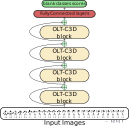
\includegraphics[width=\unitlength,page=1]{OLTC3D.pdf}}%
    \put(0.50227895,0.81646332){\makebox(0,0)[lt]{\lineheight{1.25}\smash{\begin{tabular}[t]{l}OLT-C3D\\block\end{tabular}}}}%
    \put(0,0){\includegraphics[width=\unitlength,page=2]{OLTC3D.pdf}}%
    \put(0.50227895,0.62773658){\makebox(0,0)[lt]{\lineheight{1.25}\smash{\begin{tabular}[t]{l}OLT-C3D\\block\end{tabular}}}}%
    \put(0,0){\includegraphics[width=\unitlength,page=3]{OLTC3D.pdf}}%
    \put(0.50227895,0.43900985){\makebox(0,0)[lt]{\lineheight{1.25}\smash{\begin{tabular}[t]{l}OLT-C3D\\block\end{tabular}}}}%
    \put(0,0){\includegraphics[width=\unitlength,page=4]{OLTC3D.pdf}}%
    \put(0.50227895,0.25028312){\makebox(0,0)[lt]{\lineheight{1.25}\smash{\begin{tabular}[t]{l}OLT-C3D\\block\end{tabular}}}}%
    \put(0,0){\includegraphics[width=\unitlength,page=5]{OLTC3D.pdf}}%
    \put(0.49139194,0.31989023){\makebox(0,0)[lt]{\lineheight{1.25}\smash{\begin{tabular}[t]{l}+\end{tabular}}}}%
    \put(0,0){\includegraphics[width=\unitlength,page=6]{OLTC3D.pdf}}%
    \put(0.49139194,0.50709497){\makebox(0,0)[lt]{\lineheight{1.25}\smash{\begin{tabular}[t]{l}+\end{tabular}}}}%
    \put(0,0){\includegraphics[width=\unitlength,page=7]{OLTC3D.pdf}}%
    \put(0.49139194,0.69544121){\makebox(0,0)[lt]{\lineheight{1.25}\smash{\begin{tabular}[t]{l}+\end{tabular}}}}%
    \put(0,0){\includegraphics[width=\unitlength,page=8]{OLTC3D.pdf}}%
    \put(0.49139194,0.88378744){\makebox(0,0)[lt]{\lineheight{1.25}\smash{\begin{tabular}[t]{l}+\end{tabular}}}}%
    \put(0,0){\includegraphics[width=\unitlength,page=9]{OLTC3D.pdf}}%
    \put(0.33334434,0.01010179){\makebox(0,0)[lt]{\lineheight{1.25}\smash{\begin{tabular}[t]{l}Input Images\end{tabular}}}}%
    \put(0,0){\includegraphics[width=\unitlength,page=10]{OLTC3D.pdf}}%
    \put(0.34807782,0.93918452){\makebox(0,0)[lt]{\lineheight{1.25}\smash{\begin{tabular}[t]{l}Feed Forward layers\end{tabular}}}}%
    \put(0.94817146,0.03386734){\color[rgb]{0,0,1}\makebox(0,0)[lt]{\lineheight{1.25}\smash{\begin{tabular}[t]{l}t\end{tabular}}}}%
    \put(0.90249576,0.03386734){\color[rgb]{0,0,1}\makebox(0,0)[lt]{\lineheight{1.25}\smash{\begin{tabular}[t]{l}t-1\end{tabular}}}}%
    \put(0.86178907,0.03386734){\color[rgb]{0,0,1}\makebox(0,0)[lt]{\lineheight{1.25}\smash{\begin{tabular}[t]{l}t-2\end{tabular}}}}%
    \put(0.82557281,0.0374996){\color[rgb]{0,0,1}\makebox(0,0)[lt]{\lineheight{1.25}\smash{\begin{tabular}[t]{l}...\end{tabular}}}}%
    \put(0,0){\includegraphics[width=\unitlength,page=11]{OLTC3D.pdf}}%
    \put(0.34807782,1.0182859){\makebox(0,0)[lt]{\lineheight{1.25}\smash{\begin{tabular}[t]{l}blank ∪ classes scores\end{tabular}}}}%
  \end{picture}%
\endgroup%
